\documentclass[aspectratio=169]{beamer}

% --- Pakiety językowe i kodowanie ---
\usepackage[utf8]{inputenc}
\usepackage[T1]{fontenc}

% --- Pakiety matematyczne i graficzne ---
\usepackage{amsmath, amssymb, amsfonts}
\usepackage{graphicx}
\usepackage{booktabs}

% --- Motyw i kolorystyka Beamera ---
\usetheme{Madrid}
\usecolortheme{whale}
\usefonttheme{professionalfonts}

% --- Definicje notacji kwantowej (Dirac bra-ket) ---
\newcommand{\bra}[1]{\langle #1 \rvert}
\newcommand{\ket}[1]{\lvert #1 \rangle}
\newcommand{\braket}[2]{\langle #1 \vert #2 \rangle}

% --- Informacje o prezentacji ---
\title[Algorytmy Kwantowe]{Algorytmy Kwantowe: Od Fizyki Mikroświata do Przewagi Obliczeniowej}
\subtitle{Fizyczne zjawiska, aparat przestrzeni Hilberta i algorytm Grovera}
\author[Informatyka Kwantowa]{Adam Gwiazdoń}
\date{24.11.2026}

\begin{document}

% ==============================================================================
% SLAJD 1: Tytułowy
% ==============================================================================
\begin{frame}
    \titlepage
\end{frame}

% ==============================================================================
% SLAJD 2: Spis treści
% ==============================================================================
\begin{frame}
    \frametitle{Plan prezentacji}
    \tableofcontents
\end{frame}

% ==============================================================================
% SLAJD 3: Filar Fizyczny - Podstawy mechaniki kwantowej
% ==============================================================================
\section{Filar fizyczny: Mechanika kwantowa}
\begin{frame}
    \frametitle{Filar fizyczny: Kwantowa natura informacji}
    
    \begin{block}{Zasada superpozycji stanów kwantowych}
        Podczas gdy klasyczny bit przyjmuje dyskretną wartość $0$ lub $1$, kwantowy bit (kubit) istnieje w liniowej kombinacji stanów bazowych:
        \begin{equation*}
            \ket{\psi} = \alpha \ket{0} + \beta \ket{1}, \quad \alpha, \beta \in \mathbb{C}, \quad |\alpha|^2 + |\beta|^2 = 1
        \end{equation*}
    \end{block}

    \vspace{0.3cm}
    \textbf{Kluczowe zjawiska fizyczne wykorzystywane w obliczeniach:}
    \begin{itemize}
        \item \textbf{Interferencja amplitud:} prawdopodobieństwa mogą wzmacniać stany pożądane (konstruktywna) i wygaszać błędne (destruktywna).
        \item \textbf{Postulat pomiaru (Reguła Borna):} pomiar niszczy stan superpozycji, rzutując układ na stan $\ket{x}$ z prawdopodobieństwem $P(x) = |\braket{x}{\psi}|^2$.
        \item \textbf{Dekoherencja kwantowa:} niepożądane oddziaływanie z otoczeniem prowadzące do utraty właściwości kwantowych.
    \end{itemize}
\end{frame}

% ==============================================================================
% SLAJD 4: Filar Matematyczny - Formalizm przestrzeni Hilberta
% ==============================================================================
\section{Filar matematyczny: Formalizm przestrzeni Hilberta}
\begin{frame}
    \frametitle{Filar matematyczny: Przestrzenie Hilberta i operatory}

    \begin{exampleblock}{Przestrzeń stanów i operatory unitarne}
        Stan układu kwantowego jest wektorem jednostkowym w zespolonej przestrzeni Hilberta $\mathcal{H} \cong \mathbb{C}^2$. Dopuszczalną ewolucją zamkniętego układu kwantowego są przekształcenia unitarne:
        \begin{equation*}
            U^\dagger U = U U^\dagger = I \implies \langle U\phi \mid U\psi \rangle = \braket{\phi}{\psi}
        \end{equation*}
    \end{exampleblock}

    \vspace{0.2cm}
    \textbf{Fundament obliczeń – Bramka Hadamarda ($H$):}
    \begin{equation*}
        H = \frac{1}{\sqrt{2}} \begin{pmatrix} 1 & 1 \\ 1 & -1 \end{pmatrix}, \qquad
        H \ket{0} = \frac{\ket{0} + \ket{1}}{\sqrt{2}}, \qquad
        H \ket{1} = \frac{\ket{0} - \ket{1}}{\sqrt{2}}
    \end{equation*}
    Bramka Hadamarda generuje idealnie zrównoważoną superpozycję ze stanu bazowego.
\end{frame}

% ==============================================================================
% SLAJD 5: Rejestry wielokubitowe i eksplozja wymiarowości
% ==============================================================================
\begin{frame}
    \frametitle{Rejestry wielokubitowe: Iloczyn tensorowy}

    \begin{block}{Eksplozja wymiarowości przestrzeni stanów}
        Układ złożony z $n$ kubitów opisany jest iloczynem tensorowym pojedynczych przestrzeni, osiągając wymiar $N = 2^n$:
        \begin{equation*}
            \mathcal{H}^{\otimes n} = \mathcal{H}_1 \otimes \mathcal{H}_2 \otimes \dots \otimes \mathcal{H}_n, \quad \dim(\mathcal{H}^{\otimes n}) = 2^n
        \end{equation*}
    \end{block}

    \vspace{0.2cm}
    \textbf{Generowanie równomiernej superpozycji wszystkich stanów:}
    Aplikując bramki Hadamarda na każdy z $n$ kubitów w stanie $\ket{0}$, otrzymujemy:
    \begin{equation*}
        \ket{s} = H^{\otimes n} \ket{0}^{\otimes n} = \frac{1}{\sqrt{2^n}} \sum_{x=0}^{2^n-1} \ket{x} = \frac{1}{\sqrt{N}} \sum_{x=0}^{N-1} \ket{x}
    \end{equation*}
    \begin{itemize}
        \item Równoczesne kodowanie informacji o $2^n$ stanach w zaledwie $n$ fizycznych cząstkach.
        \item Podstawa kwantowego paralelizmu – algorytm manipuluje całą sumą w jednym kroku.
    \end{itemize}
\end{frame}

% ==============================================================================
% SLAJD 6: Filar Algorytmiczny - Problem przeszukiwania
% ==============================================================================
\section{Filar algorytmiczny: Algorytm Grovera}
\begin{frame}
    \frametitle{Filar algorytmiczny: Problem przeszukiwania bazy}

    \begin{alertblock}{Klasyczne ograniczenie przeszukiwania}
        Dla niestrukturyzowanej bazy $N = 2^n$ elementów poszukujemy unikalnego $\omega$ spełniającego warunek wyroczni: $f(\omega) = 1$ oraz $f(x) = 0$ dla $x \neq \omega$.
        \begin{itemize}
            \item Najgorszy przypadek klasyczny: $N$ zapytań do funkcji testującej.
            \item Przypadek średni: $\frac{N}{2}$ zapytań $\implies$ złożoność $\mathcal{O}(N)$.
        \end{itemize}
    \end{alertblock}

    \vspace{0.2cm}
    \textbf{Wyrocznia kwantowa (Quantum Oracle):}
    Działa jako operator unitarny $U_\omega$ odwracający fazę wyłącznie szukanego stanu:
    \begin{equation*}
        U_\omega \ket{x} = (-1)^{f(x)} \ket{x} = I - 2\ket{\omega}\bra{\omega}
    \end{equation*}
    Wartość szukana jest oznaczana ujemną amplitudą, podczas gdy reszta stanów pozostaje nienaruszona.
\end{frame}

% ==============================================================================
% SLAJD 7: Przebieg procedury algorytmu Grovera
% ==============================================================================
\begin{frame}
    \frametitle{Przebieg procedury algorytmu Grovera}

    \textbf{Kolejne kroki algorytmu (Quantum Search Protocol):}
    \begin{enumerate}
        \item \textbf{Inicjalizacja rejestru:} Przygotowanie $n$ kubitów w stanie bazowym $\ket{0}^{\otimes n}$.
        \item \textbf{Utworzenie superpozycji:} Zastosowanie transformaty Hadamarda: $\ket{s} = H^{\otimes n}\ket{0}^{\otimes n}$.
        \item \textbf{Pętla iteracji Grovera:} Wykonanie $R \approx \frac{\pi}{4}\sqrt{N}$ powtórzeń operatora $G$:
        \begin{equation*}
            G = D \cdot U_\omega, \quad \text{gdzie } D = 2\ket{s}\bra{s} - I
        \end{equation*}
        \item \textbf{Pomiar końcowy:} Odczytanie rejestru w standardowej bazie obliczeniowej.
    \end{enumerate}

    \begin{block}{Operator dyfuzji Grovera (Inwersja wokół średniej)}
        Operator $D = 2\ket{s}\bra{s} - I$ odbija amplitudy stanów względem ich bieżącej wartości średniej, zamieniając ujemną amplitudę stanu $\ket{\omega}$ na gwałtowny wzrost prawdopodobieństwa.
    \end{block}
\end{frame}

% ==============================================================================
% SLAJD 8: Dwie kolumny + grafika (Interpretacja geometryczna)
% ==============================================================================
\begin{frame}
    \frametitle{Interpretacja geometryczna iteracji Grovera}

    \begin{columns}[c]
        % Kolumna 1: Opis matematyczno-fizyczny
        \begin{column}{0.50\textwidth}
            \begin{block}{Dynamika w podprzestrzeni 2D}
                Cała dynamika algorytmu rozgrywa się na płaszczyźnie rozpiętej przez stan $\ket{\omega}$ oraz stan reszty bazy $\ket{\omega^\perp} = \frac{1}{\sqrt{N-1}}\sum_{x \neq \omega} \ket{x}$:
                \begin{itemize}
                    \item Kąt początkowy: $\sin(\theta/2) = \frac{1}{\sqrt{N}}$.
                    \item Wyrocznia $U_\omega$ odbija wektor względem osi $\ket{\omega^\perp}$.
                    \item Dyfuzor $D$ odbija wektor względem $\ket{s}$.
                    \item Złożenie dwóch odbić to \textbf{czysty obrót} o stały kąt $\theta \approx \frac{2}{\sqrt{N}}$ w kierunku stanu $\ket{\omega}$.
                \end{itemize}
            \end{block}
        \end{column}

        % Kolumna 2: Załączony obrazek
        \begin{column}{0.48\textwidth}
            \centering
            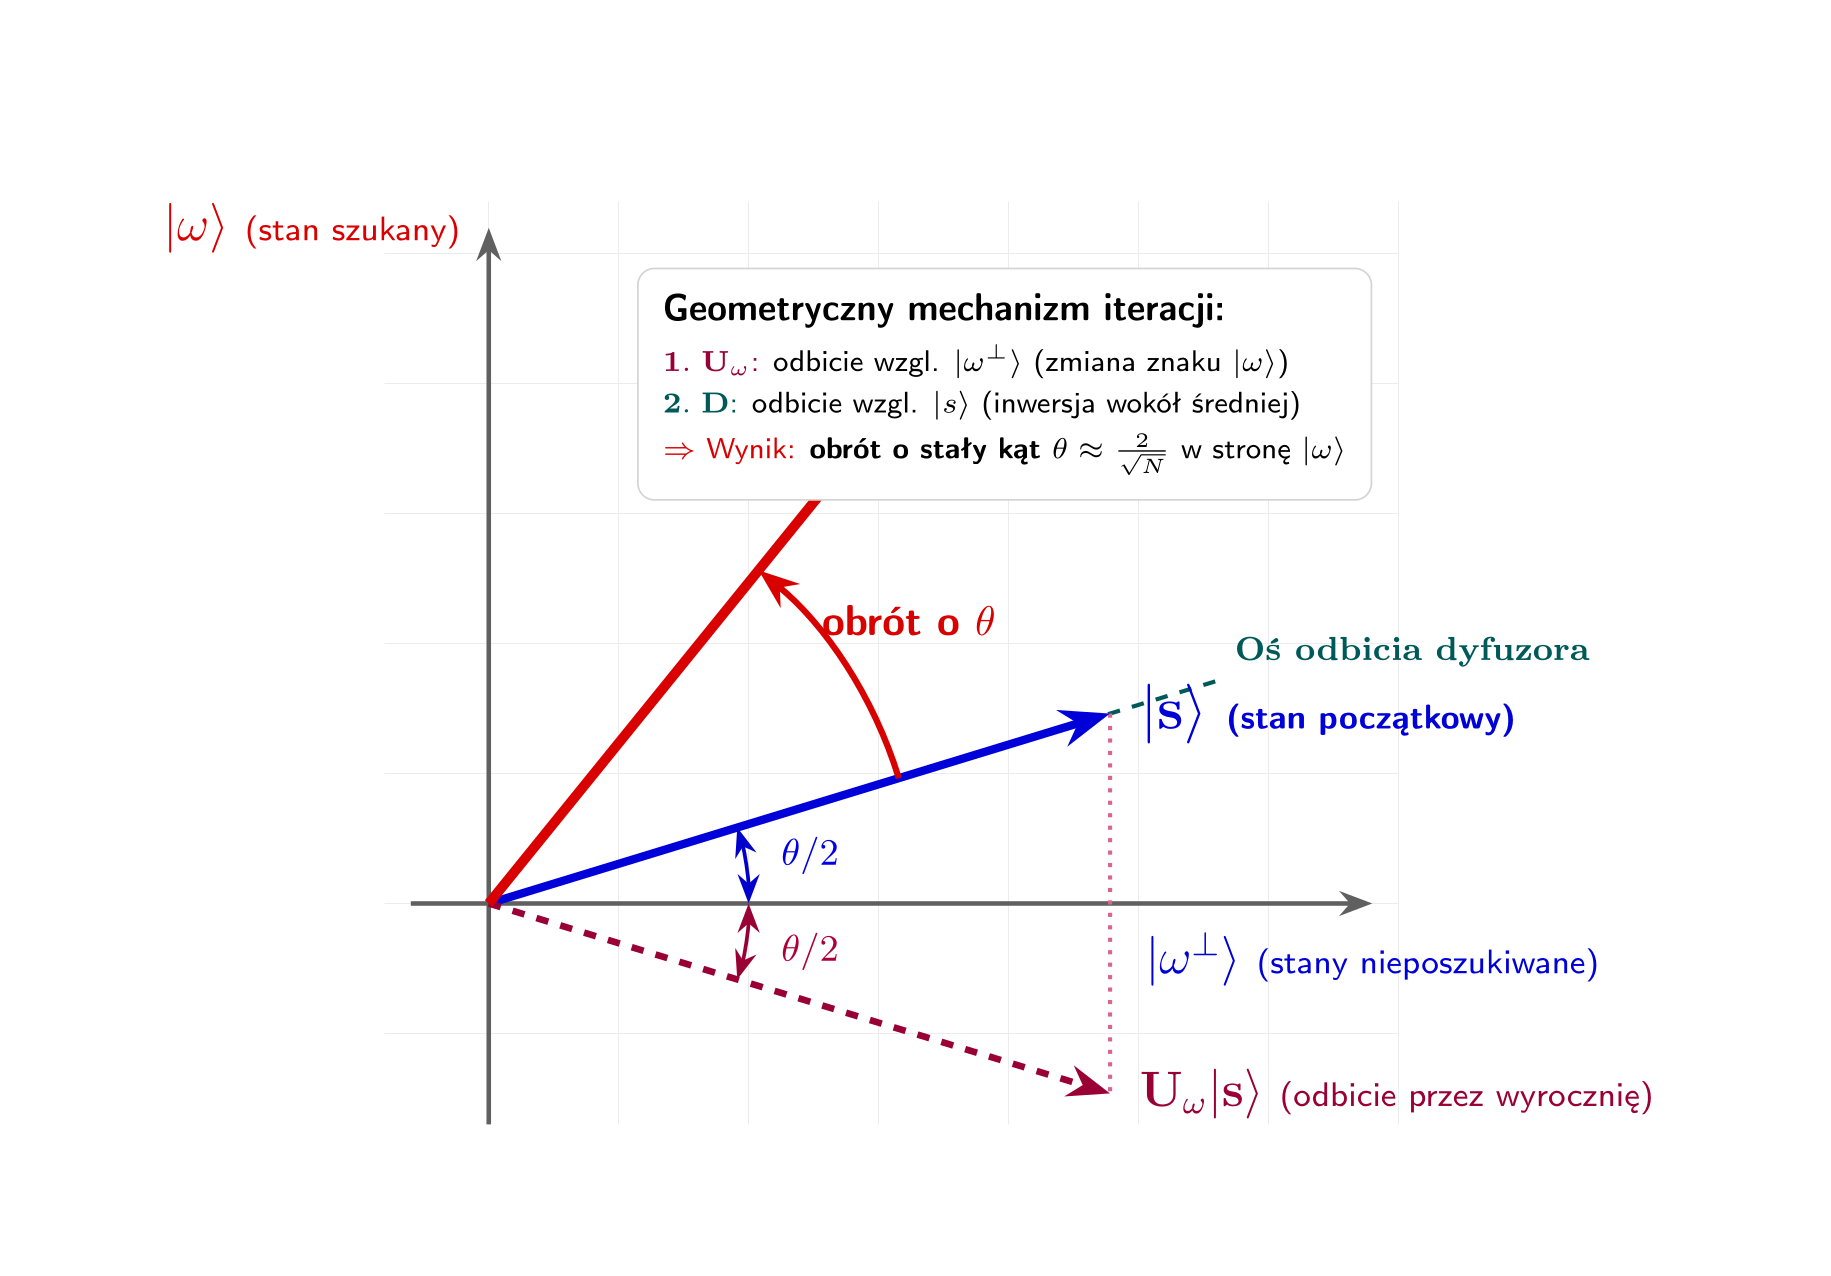
\includegraphics[width=\linewidth]{grover_diagram.png}
            \vspace{0.1cm}
            {\footnotesize \textbf{Rysunek:} Odbicia i rotacja wektora stanu w stronę rozwiązania $\ket{\omega}$.}
        \end{column}
    \end{columns}
\end{frame}

% ==============================================================================
% SLAJD 9: Złożoność obliczeniowa i przewaga kwantowa
% ==============================================================================
\section{Złożoność i podsumowanie}
\begin{frame}
    \frametitle{Złożoność obliczeniowa i przewaga kwantowa}

    \begin{exampleblock}{Przyspieszenie kwadratowe (Quadratic Speedup)}
        Liczba wymaganych iteracji do osiągnięcia prawdopodobieństwa sukcesu bliskiego $1$:
        \begin{equation*}
            R \approx \frac{\pi}{4}\sqrt{N} \implies \mathcal{O}(\sqrt{N}) \quad \text{vs.} \quad \mathcal{O}(N) \text{ (klasycznie)}
        \end{equation*}
    \end{exampleblock}

    \vspace{0.2cm}
    \textbf{Porównanie w skali rzeczywistej ($N = 10^{12}$ – bilion elementów):}
    \begin{itemize}
        \item \textbf{Komputer klasyczny:} $\approx 5 \cdot 10^{11}$ operacji (godziny/dni obliczeń).
        \item \textbf{Algorytm Grovera:} $\approx \frac{\pi}{4} \cdot 10^6 \approx 785\,398$ operacji (ułamek sekundy).
    \end{itemize}

    \begin{alertblock}{Optymalność twierdzenia BBBV}
        Dowód Bennetta, Bernsteina, Brassarda i Vaziraniego (1997) udowadnia, że żaden algorytm kwantowy nie może przeszukać czarnej skrzynki szybciej niż w czasie $\Omega(\sqrt{N})$. Algorytm Grovera jest zatem ściśle optymalny!
    \end{alertblock}
\end{frame}

% ==============================================================================
% SLAJD 10: Podsumowanie i wnioski
% ==============================================================================
\begin{frame}
    \frametitle{Podsumowanie i perspektywy rozwoju}

    \begin{block}{Synteza trzech dyscyplin naukowych}
        \begin{itemize}
            \item \textbf{Fizyka:} dostarcza zjawiska superpozycji i konstruktywnej interferencji.
            \item \textbf{Matematyka:} formalizuje ewolucję w przestrzeniach Hilberta poprzez transformacje unitarne i obroty geometryczne.
            \item \textbf{Algorytmika:} optymalizuje ścieżkę obliczeń, gwarantując zysk $\mathcal{O}(\sqrt{N})$.
        \end{itemize}
    \end{block}

    \vspace{0.1cm}
    \textbf{Współczesne implikacje i wyzwania:}
    \begin{itemize}
        \item \textbf{Kryptografia symetryczna:} konieczność podwojenia długości kluczy (np. AES-256 zamiast AES-128).
        \item \textbf{Architektury NISQ:} realizacja wymaga kwantowej korekcji błędów (QEC).
    \end{itemize}

    \vspace{0.1cm}
    \begin{center}
        \textbf{\large Dziękuję za uwagę!} \\
        {\footnotesize Pytania i dyskusja}
    \end{center}
\end{frame}

\end{document}
